% main.tex, to be used with thesis.tex
% This contains the main work of your thesis.

%\bibliography{thesis}  % uses the references stored in Chapter1Radar.bib

\chapter{DSP Data Persistence: Component Design and Architecture}

The mongoDB database system was selected, as stated in Chapter 5, to store 
the collected data from the SF-BEAMS sensor network. NetBEAMS is based on a 
component-based architecture, where each of the components can play different
roles during their lifecycle. It uses the abstraction of Data Producers and 
Data Consumers: while a component produces data to the system, the latter 
consumes \cite{netbeams2009}. In this way, a DSP Data Component was designed
and implemented to provide the integration between NetBEAMS and the mongoDB 
database. This integration is based on the Data Sensor Platform (DSP), the
kernel software stack provided by NetBEAMS, as documented in
\cite{netbeams-dsp-architecture}. 

This chapter follows the steps taken in Software Engineering guidelines to
analyze and design a software component using Object-Oriented Analysis and 
Design \cite{oop} using the techniques from the Agile and XP Scrum
\cite{agile-scrum} processes. First, Section \ref{sec:business-process-analysis} gives an
overview of the problem by analyzing a basic scenario of the data collection process used in NetBEAMS.
Then, the Section \ref{sec:requirements-specs} describes the requirements for
the design of the new component, followed by the specifications of the data
model used for the mongoDB database in Section
\ref{sec:dsp-persistence-data-model}. Lastly, the high-level architecture
of Section \ref{sec:system-architecture} gives the foundation of the
DSP Data Persistence component design of Section \ref{sec:dsp-data-comp-design}.

Details about the implementation of this design are located in the
Appendix Section \ref{sec:dsp-data-persistence-implementation}.

\section{Business Process Analysis}
\label{sec:business-process-analysis}

As described in \cite{netbeams-dsp-architecture}, the DSP Platform was designed
to support SF-BEAMS. As shown in Figure \ref{fig:dsp-persistence-business-process}, 
the event of data collection starts by the DSP Component deployed on each 
DSP Gateway Node \cite{netbeams-dsp-architecture}, by the event ``Measurements
X Collected''. When this DSP Client component finishes the data extraction
process, a new one starts. First, each of the co-located DSP Client processes 
the collected measurements and creates a DSP Message, embodying the collected 
data from the associated sensor device. Each DSP Message is added into a local
temporary outbound queue that waits to be transmitted. Then, an asynchronous 
data transmission event occurs at a specified rate, packaging all DSP
Messages into the body of a DSP Messages Container in order to be serialized
into XML (shown in Listing \ref{stream:dsp-message-serialized-ysi} on page
\pageref{stream:dsp-message-serialized-ysi}) and transferred to the DSP Server
host, a centralized server that receives all the collected data embodied into each of the DSP Messages.

\begin{figure}[!b]
  \centering
  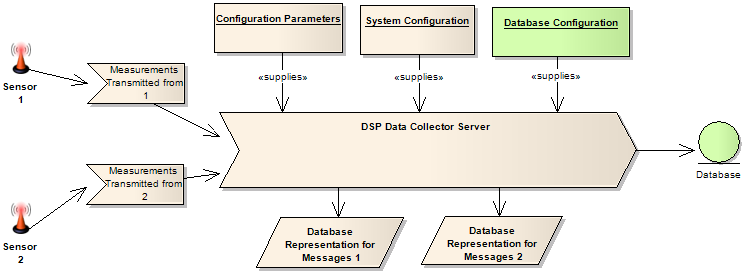
\includegraphics[scale=0.6]{../diagrams/DSP-DataPersistence-Business-Diagram}
  \caption{UML Business Process Model diagram - Adding Persistence for NetBEAMS}
  \label{fig:dsp-persistence-business-process}
\end{figure}

The goal of the new DSP Data Persistence component is to proxy the payload 
from the DSP Messages to the new suggested Measurements Database. Once the DSP
Server receives all the messages in a container, it processes the messages and
sends their payloads to the Measurements Database. This process requires a new
Database Configuration to be provided to the DSP Server host, as well as the
installation and setup of the new Measurements Database. In this way, different
users of the collected data, such as Programmers and Biologists, can access the
collected data directly from the Measurements Database and reuse them by
Exporting specific observation parameters to different formats of their
interest.

\section{Requirements Specification}
\label{sec:requirements-specs}
This section outlines the functionalities and constraints that the developed
solution must perform and follow, respectively, obtained by analyzing the main
data collection scenario described in the previous section and reviewing the
requirements defined by the RTC staff members.

\subsection{Functional Requirements}
\label{sec:use-cases}

The primary goal of the system is to allow users to have easy access to the 
collected data from \emph{NetBEAMS} using a schema-less database technology.
mongoDB provides access to the stored data without requiring the use of 
a Structured Query Language. Instead, that technology provides a programming
language abstraction that makes the access to the stored data easier 
\cite{sn-programming-language}. Using Agile User Stories to describe Use 
Cases Diagrams \cite{use-cases-user-stories}, Figure 
\ref{fig:DSP-Data-Persistence-UseCases-Diagram-Users} enumerates these
functionalities as customers conversations, starting with a fictitious
persona, the action it desires to perform and the outcome of the action, a
requirements gathering pattern defined in Scrum \cite{agile-scrum}:

\begin{figure}[!b]
  \centering
  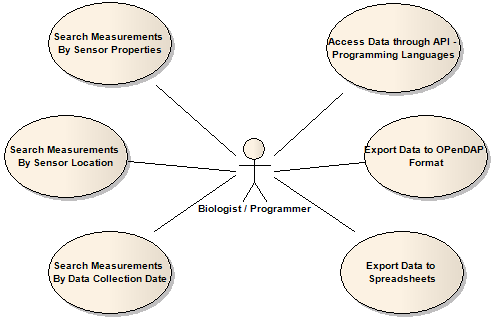
\includegraphics[scale=0.65]{../diagrams/DSP-Data-Persistence-UseCases-Diagram-Users}
  \caption{UML Use Case diagram for Persistence Functions}
  \label{fig:DSP-Data-Persistence-UseCases-Diagram-Users}
\end{figure}

\begin{itemize}
  \item \textbf{Search Measurements by Sensor Properties}: "As a marine
  biologist, I would like to search observations by filtering values of the 
  sensor device's properties such as temperature or salinity, so that I can 
  find specific associated values to the observation.";
  \item \textbf{Search Measurements by Sensor Location}: "As an oceanographer,
  I would like to search observations that took place at the geographic
  coordinates (x latitude, y longitude), so that I can assess the area around
  the given coordinates.";
  \item \textbf{Search Measurements by Data collection date}: "As a marine 
  biologist, I would like to search observations that took place last week, 
  so that I can assess past environmental conditions";
  \item \textbf{Annotate Existing Measurements}: "As a estuarine ecologist,
  I would like to annotate observations from the time the oil spill occurred
  in the San Francisco Bay, so that I can maintain historical evidence of 
  the impact of such event.";
  \item \textbf{Export Data to Spreadsheets}: "As a scientist from RTC, I 
  would like to analyze of the observed data from yesterday using a 
  spreadsheet, so that I can verify measurements using Microsoft Excel.";
  \item \textbf{Export Data to OPeNDAP format}: "As a biologist, I would 
  like to export the collected data produced during this month using the
  OPeNDAP data format, so that I can collaborate with other research groups
  that use this data format.";
  \item \textbf{Access the data through API, Programming Languages}: "As a
  marine biologist who learned the Python scripting language, I would like to
  write a software that connects directly to the database, so that I can
  implement a customized analysis system for NetBEAMS.";
  \item \textbf{Remove Undesired Measurements}: "As an oceanographer, I
  would like to remove specific observations collected yesterday, 
  so that the research group does not use 'junk data'.".
\end{itemize}

As one can see, the basic users' functionalities are related to the access to
the collected data using different parameters related to the each observation's
properties or implied metadata such as time of collection or location. In order
to do so, the functions to be performed were developed following the
specifications of the Data Sensor Platform (DSP) architecture, as described in
\cite{netbeams-dsp-architecture}. In order to collect data sent to the NetBEAMS
server, the new DSP component must act as a Data Consumer. The functionalities
provided by this component can be seen in the UML Use Cases diagram \cite{uml}
in Figure \ref{fig:DSP-Data-Persistence-UseCases-Diagram-System}, and
summarized as follows:

\begin{figure}[!h]
  \centering
  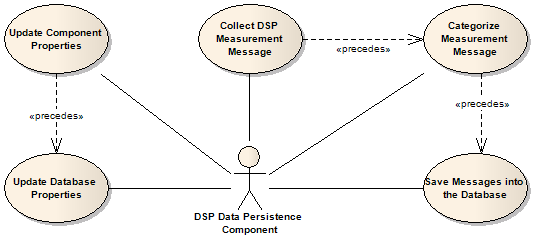
\includegraphics[scale=0.65]{../diagrams/DSP-Data-Persistence-UseCases-Diagram-System}
  \caption{UML Use Case diagram for the Persistence Component}
  \label{fig:DSP-Data-Persistence-UseCases-Diagram-System}
\end{figure}

\begin{itemize}
  \item \textbf{Update Component Properties}: the component must be
  configurable, with its own set of properties, such as the flush rate used 
  to send data to the database system;
  \item \textbf{Update Database Properties}: the component must be able to
  update the mongoDB database settings such as IP Address and  communication 
  port;
  \item \textbf{Collect DSP Measurement Message}: the component must be
  able to receive and temporarily retain the collected messages from
  different the sensors devices;
  \item \textbf{Categorize Measurement Message}: the component must be able
  to categorize the DSP Message, as it arrives, by its properties such as 
  transaction time, and originating DSP Message ID;
  \item \textbf{Save Messages into the Database}: the component must be able
  to send the payload of the DSP Messages to the database.
\end{itemize}

\subsection{Non-Functional Requirements}

Different constraints were required to execute the functional requirements
described in the previous section. Those constraints are listed as different
non-functional requirements as follows:

\begin{itemize}
  \item The solution must maintain the received DSP Measurement Messages
  in-memory for a specific period of time in order to decrease the write load
  on the database (flush rate);
  \item The persistence storage system must be able to cope with the Data
  Volume produced by SF-BEAMS on daily basis;
  \item The persistence storage system must be able to scale without minimal
  architectural and schema changes;
  \item The persistence storage system must be able to provide access to the
  persisted data using an programmatic abstraction interface, as the authors
  of \cite{sn-programming-language} proposed.
\end{itemize}

Driven by the requirements defined, the definition of the keys of the key-value
pairs model, used to describe the collected data from the sensor devices and
their associated metadata, is the foundation for the integration between the
DSP Data Persistence component and the mongoDB database. Next section details
the data model design that specifies those keys.

\section{Data Model Design}
\label{sec:dsp-persistence-data-model}

MongoDB is defined as a Document-Oriented Database system, which is based on 
the abstraction of the Key-Value-Pair data model, using a binary version of JSON
\cite{json} as its main data representation. MongoDB does not require the creation 
of a database schema, rather the definition of keys that comprise a document on
the database organized into separate collections of relating documents. In
order to describe the keys of a document, the guidelines provided by the Data
Provenance taxonomy was used. The key-value pairs of any instance of the
collected data must include the following key properties:

\begin{itemize}
  \item \textbf{Location}: properties that describe the location of the data.
  For example, the host machine name, IP address, or the GPS coordinates
  \cite{gps} from the sensor device;
  \item \textbf{Identity}: what uniquely identifies the data among 
  others, produced by other sensor devices in the network such as the DSP
  Message ID using UUID\footnote{Universally Unique Identifier};
  \item \textbf{Time-Dimensions}: when the data was recorded 
  \cite{db-provenance} and when the transaction occurred \cite{sn-time-series}.
\end{itemize}

After analyzing the DSP Message Structure, as well as the YSI Sonde Data
Handler of the DSP Platform architecture documentation
\cite{netbeams-dsp-architecture}, the design of the document developed to
identify both the data and metadata of the collected data is organized as
follows:

\begin{itemize}
  \item \textbf{message\underline{ }id}: Defines the DSP Message ID that
  carried the observation from the sensor device to the DSP Server. This ID
  can be used during network and database inspections in order to track messages
  for the DSP Platform;
  \item \textbf{sensor}: Defines the properties of the sensor device;
    \begin{itemize}[label=\textbullet]
        \item \textbf{ip\underline{ }address} Defines the IP Address of the 
        sensor device that produced the data;
        \item \textbf{location}: Defines the geographical coordinates of the
        sensor device, using the Decimals Degree format \cite{decimal-degrees};
            \begin{itemize}[label=\textbullet]
                \item \textbf{latitude} the GPS latitude coordinate of the
                position of the sensor device;
                \item \textbf{longitude}: the GPS longitude coordinate of the
                position of the sensor device.
            \end{itemize}
    \end{itemize}
  \item \textbf{time}: Defines different time dimensions according to Data 
   Provenance;
    \begin{itemize}[label=\textbullet]
      \item \textbf{valid}: it is extracted from the container's date and time
      of creation, which was collected during the sensor device's reading;
      \item \textbf{transaction}: it is extracted from the DSP message
         container's creation time and it is used to identify when the
         transaction, which transferred the message from the DSP Gateway Client
         to the DSP Server, occurred;
    \end{itemize} 
    \item \textbf{observation}: carries the observations of a given sensor
    device. For example, the observation key of for the YSI device
    \cite{YSI-Sonde} may contains all the subsets of the properties defined
    for the device, such as battery, temperature and salinity, among others.
\end{itemize}

MongoDB uses JSON data structure \cite{json} to represent a document, as the
example shown in Figure \ref{fig:kvp-json-viewer} on page
\pageref{fig:kvp-json-viewer}. Any number of keys can be in the root branch of
the tree, as well as in sub branches of the document structure. The values of
the tree are concentrated in the leaves of the tree. Listing
\ref{file:mongodb-ysi-data-format}, on page
\pageref{file:mongodb-ysi-data-format}, shows the instance of this design on
mongoDB database. Based on this foundation, the design of the DSP Data
Persistence component evolved from a top-down approach to meet this data model
design.

\begin{figure}[!h]
  \centering
  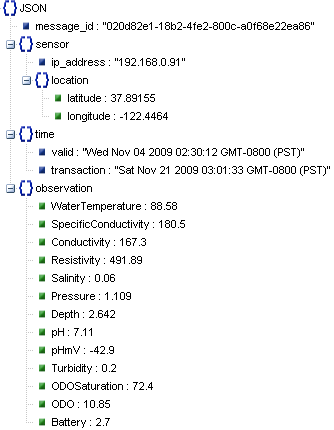
\includegraphics[scale=0.65]{../diagrams/kvp-json-viewer}
  \caption{Data Design using JSON Data Structure}
  \label{fig:kvp-json-viewer}
\end{figure}

It is important to note that mongoDB does not use any structure language, like
the use of the SQL in relational databases, to access the persisted data. In
order to access the values of the documents, the ``dot notation''
\cite{db-mongo-data-access} is used to reach each of the tree nodes. For
example, the use of ``observation.WaterTemperature'' and
``sensor.location.latitude'' give the values of the data ``water temperature'' and
the metadata ``latitude'' of the collected data, respectively.

\section{High-Level System Architecture}
\label{sec:system-architecture}

Considering the business analysis described in Section
\ref{sec:business-process-analysis}, the addition of a data persistence layer
to the DSP Platform can be achieved by adding a Data Consumer (DC) as 
described by \cite{netbeams-dsp-architecture}. Based on the 
Requirements specification, this component must be responsible for the 
extraction process that takes the payload of the body of a filtered DSP
Measurement Message and converts it to the key-value data model defined
in the previous section. This process guarantees that the collected data is
inserted to a running mongoDB database system and covers the use cases
defined. Figure \ref{fig:NetBEAMS-Persistence-Server-Node-Components}
provides an architectural overview of the DSP Server node with the
loosely-coupled components, highlighting the inclusion of a new DSP Component
called ``DSP Data Persistence''.

\begin{figure}[!h]
  \centering
  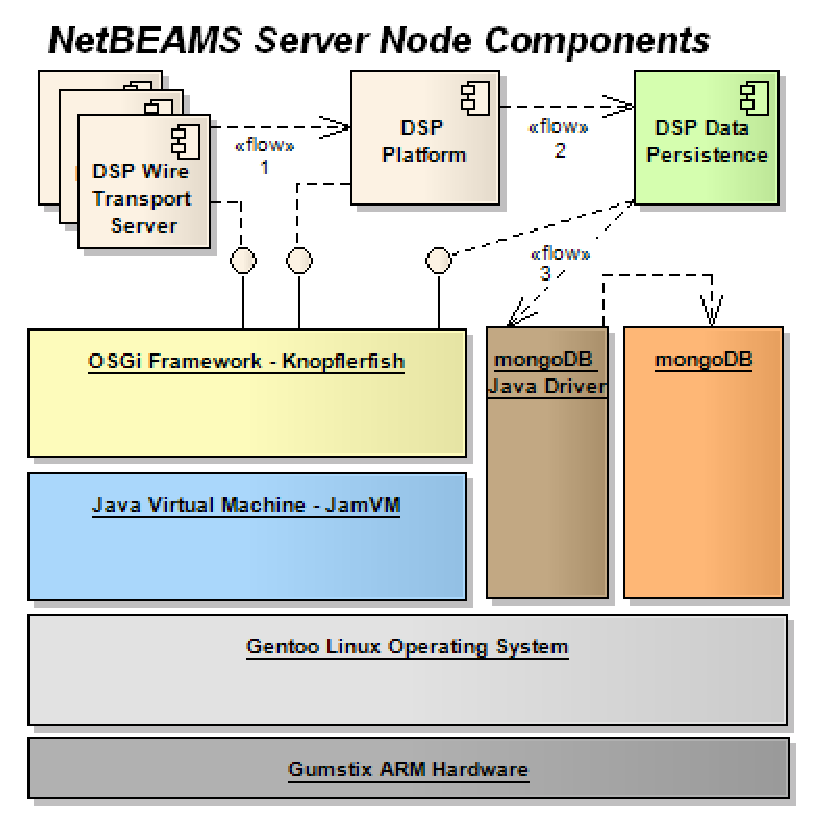
\includegraphics[scale=0.65]{../diagrams/NetBEAMS-Persistence-Server-Node-Components}
  \caption{UML Components diagram of the DSP Data Collector}
  \label{fig:NetBEAMS-Persistence-Server-Node-Components}
\end{figure}

As it is depicted the diagram 
\ref{fig:NetBEAMS-Persistence-Server-Node-Components}, the DSP Data
Persistence can be added into the existing architecture as an 
independent plug-and-play component. The database system and the necessary
drivers are also added without any changes to the existing DSP 
infrastructure. First, the DSP Messages are delivered to the DSP server 
through the DSP Wire Transport Server, as shown by flow 1. Next, the DSP 
Platform is responsible to forward a copy of the Measurement messages 
directly to the DSP Data Persistence as shown by flow 2. Then, the sole 
responsibility of the DSP Data Persistence is to transfer the received 
measurement messages to the database system by using the connection 
drivers, as shown by flow 3.

Any DSP Component is essentially an OSGi Bundle \cite{osgi-intro}, a unit of
deployment in a Java JAR format \cite{java-tutorial} containing the Java
classes and a descriptor manifest artifact that identifies the major components
of the package, which services the component requires to use and which ones it
will optionally publish during its activation and lifecycle. Details about the
deployment of the DSP Data Persistence component, as well as about the OSGi
environment used, are given in the Appendix section
\ref{sec:dsp-component-osgi-deployment}.

The following sections focus on the DSP Data Persistence component 
design in the context of an OSGi bundle \cite{osgi}.

\section{DSP Data Persistence Component Design}
\label{sec:dsp-data-comp-design}

The proposed Data Persistence component must follow the DSP Component
requirements, which specifies the design-pattern of Data Producer and Consumer
mentioned earlier in this chapter. As seen in the UML Package  Dependency
Diagram in Figure \ref{fig:DSP-Data-Persistence-Packages-Dependency}, a new
DSP Component has dependencies on three different packages: the OSGi Framework
and the DSP Platform responsible to integrate a new component into the
micro-kernel, and the mongoDB Java driver API that connects to the mongoDB
server.

\begin{figure}[!h]
  \centering
  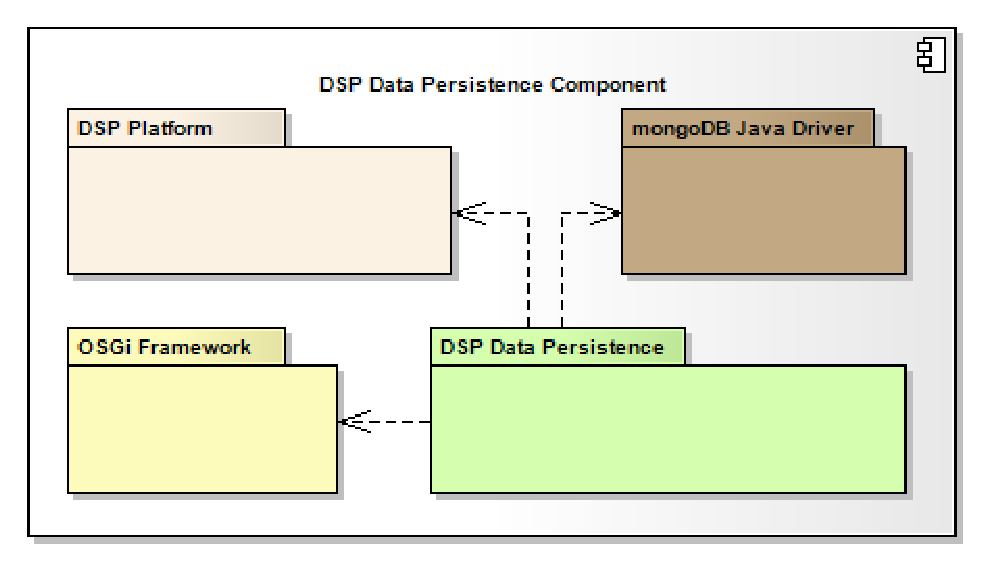
\includegraphics[scale=0.65]{../diagrams/DSP-Data-Persistence-Packages-Dependency}
  \caption{UML Components diagram of the DSP Data Collector}
  \label{fig:DSP-Data-Persistence-Packages-Dependency}
\end{figure}

In order to use a DSP Component, one must first activate it into the OSGi
Framework the DSP Platform runs on. Both the activation and the design of how
the new component acts as a Data Consumer is explained in the following
sections.

\subsection{DSP Data Persistence Activation and Message Delivery}

The DSP Data Persistence component starts with an OSGi Activator class, and 
the implementation of the DSP Component, responsible for providing services 
to the platform \cite{netbeams-dsp-architecture}. Based on these 
specifications, the following set of classes, shown in Figure 
\ref{fig:DSP-DataPersistence-Activator-Class-Diagram}, depicts the implemented
classes for the new DSP Data Persistence component.

\begin{figure}[!h]
  \centering
  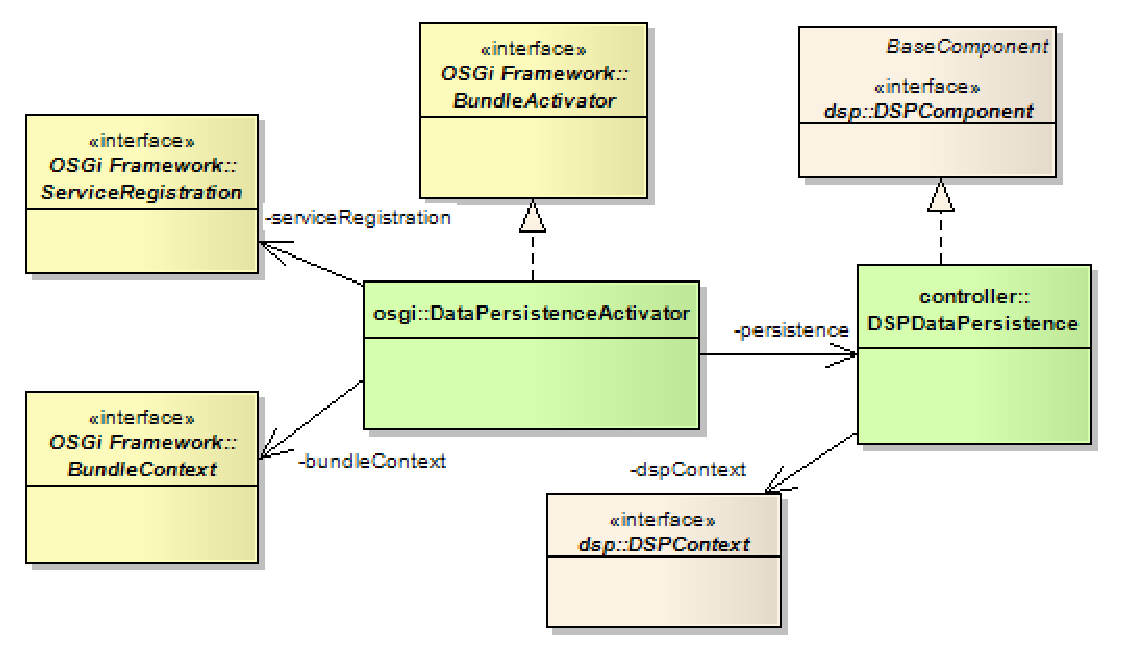
\includegraphics[scale=0.65]{../diagrams/DSP-DataPersistence-Activator-Class-Diagram}
  \caption{UML Class diagram for the DSP Data Persistence Activator and Component}
  \label{fig:DSP-DataPersistence-Activator-Class-Diagram}
\end{figure}

The class DSPDataPersistenceActivator is the main class responsible for the
activation of the class DSPDataPersistence, as it extends from the OSGi
class BundleActivator. The BundleActivator maintains references to the classes
BundleContext and ServiceReference, both from the OSGi Framework, in order to
maintain the component managed by the OSGi Framework and register the class
DSPDataPersistence as a service to the OSGi environment. Therefore, the class
DSPDataPersistenceActivator is the main communication interface between the 
DSP Platform and the OSGi Framework, are responsible for the orchestration of
the application lifecycle.

The class DSPDataPersistence implements the interface DSPComponent, responsible
to provide the contract between the component and the DSP platform. As a
consequence, this class inherits all the behavior described in
\cite{netbeams-dsp-architecture} necessary to be executed in the DSP Platform
in a given context (through the instance of class DSPContext). The different
roles played by the class DSPDataPersistence are defined as follows:

\begin{itemize}
  \item \textbf{Data Consumer}: receives any measurement message from remote
  sensors;
  \item \textbf{Data Producer}: transforms any received measurement message
  into the format defined in Section \ref{sec:dsp-persistence-data-model}, in
  order to be sent to the database.
\end{itemize}

The class DSPDataPersistenceActivator is responsible for starting and stopping,
the services provided by the DSPDataPersistence component, as this behavior is
inherited from the OSGi class BundleActivator from the OSGi Framework. Following
the specification of the DSP Architecture \cite{netbeams-dsp-architecture},
Figure
\ref{fig:From-OSGi-Framework-to-DSP-Data-PersistenceActivator-Sequence-Diagram} 
shows a UML Sequence Diagram that depicts the steps of the activation of the
DSP component, and summarized as follows:

\begin{figure}[!h]
  \centering
  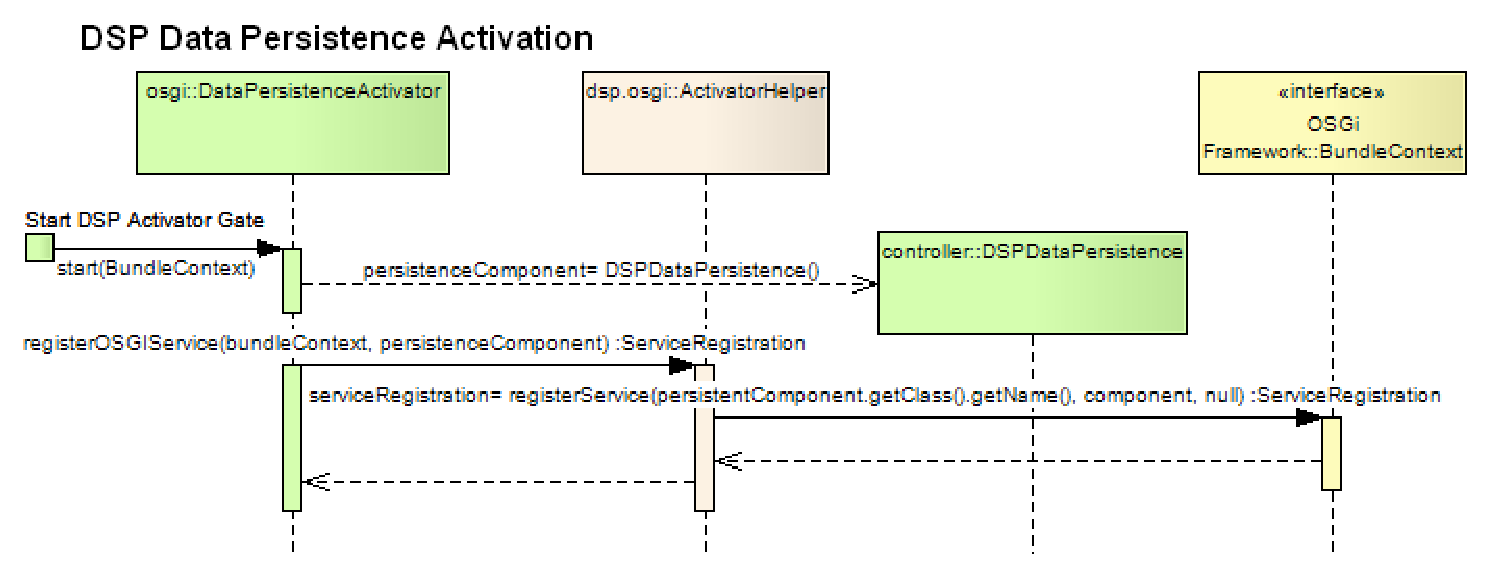
\includegraphics[scale=0.65]{../diagrams/From-OSGi-Framework-to-DSP-Data-PersistenceActivator-Sequence-Diagram}
  \caption{UML Sequence diagram describing the DSP Data Persistence bundle activation}
  \label{fig:From-OSGi-Framework-to-DSP-Data-PersistenceActivator-Sequence-Diagram}
\end{figure}

\begin{enumerate}
  \item During its activation, the DSP Platform will get the name of the
  DSP Data Persistence component from the configuration artifact config.xml as
  seen in Listing \ref{file:dsp-config.xml} on page
  \pageref{file:dsp-config.xml};
  \item After being selected based on the configuration priority, the 
  DSPBundle artifact is identified and installed by creating an instance of the
  class DSPDataPersistenceActivator, making a call to the method start();
  \item During the activation, an instance of the class DSPDataPersistence
  is created and registered as an OSGi Service;
  \item Upon registering the DSP Data Persistence component, the DSP Platform
  listens for the event serviceUpdate() and triggers the last operations to
  bootstrap the DSP Component:
   \begin{enumerate}
      \item Initialize the component by calling the method initComponent();
      \item Start the component by calling the method startComponent();
      \item Bootstrap messages by calling the method delivery(). This is where
      both the DSP Measurements Messages and Update Messages are delivered by
      the DSP Broker. This concept is based on the listener of Observer
      Design-Pattern \cite{gof}.
   \end{enumerate}
\end{enumerate}

Any configuration parameter required by a DSP Component is sent during its
bootstrap process through the use of an optional DSP Update Message, as shown
in Listing \ref{file:dsp-data-persistence-bootstrap.xml} on page
\pageref{file:dsp-data-persistence-bootstrap.xml}. The initialization of the
DSP Component Activator and the DSP Component registration are also shown in
Figure
\ref{fig:From-OSGi-Framework-to-DSP-Data-PersistenceActivator-Sequence-Diagram}.

As soon as the process "Start DSP Activator Gate" is executed, an instance of
the class DSPDataPersistence component is created to be registered into the
OSGi Framework using the DSP Platform's helper class ActivationHelper. It is
responsible to proxy the method call to the class BundleContext, which makes
the actual registration of the DSPDataPersistence component as an OSGi
Service. At this point, the DSPDataPersistence is installed and on the state
"Active", as defined by the OSGi Framework (Refer to
\cite{netbeams-dsp-architecture} for details).

Once the DSP Data Persistence component is concurrently running with other
components from both the DSP Platform and the OSGi Framework, it is able to
receive DSP Messages. The following section will explain how to bootstrap the
DSP Data Component in order to receive Measurement Messages.

\subsection{Delivering Bootstrap and Measurement Messages}

Although the DSP Data Persistence component has been instantiated as of Figure
\ref{fig:From-OSGi-Framework-to-DSP-Data-PersistenceActivator-Sequence-Diagram}, 
the process of delivering messages to the DSP Data Persistence component has yet
to be completed. As defined by the requirements, the DSP Component must execute its
function concurrently, using the configuration parameters during its
bootstrap process. The DSP Platform delivers any bootstrap message defined in
the DSP Platform runtime environment, as explained in the Appendix section
\ref{sec:dsp-persistence-boostrap}. However, to deliver DSP Measurement
Messages, a new filter must be provided. As explained in
\cite{netbeams-dsp-architecture}, the DSP Broker uses the DSP Matcher's rules
to select to Data Consumers configured in a given DSP. For this reason, a rule
that filters any remote measurement message received by running DSP Server is
used, as shown in Listing \ref{file:dsp-matcher-config.xml} on page
\pageref{file:dsp-matcher-config.xml}. The rule defined in line 63 express
that all messages created by any producer on any DSP Host, either client or
sever, has as delivery target the DSP Data Persistence component. In this way,
when DSP Measurement Messages are delivered, the DSP Broker delivers the DSP
Message to the DSP Data Persistence Component.

The UML Class Diagram for the participating classes of the DSP Data
Persistence component is shown in Figure
\ref{fig:DSP-DataPersistence-Flusher-Classes}. The class DSPDataFlusher is
responsible for running as a worker thread, whose function is to verify if
there are messages to be flushed to the Database by contacting the Singleton
class \cite{gof} TransientPersistenceLayer, responsible to keep track of the
DSP Messages received when the DSP Broker delivered them to the DSP Data
Persistence component.

\begin{figure}[!h]
  \centering
  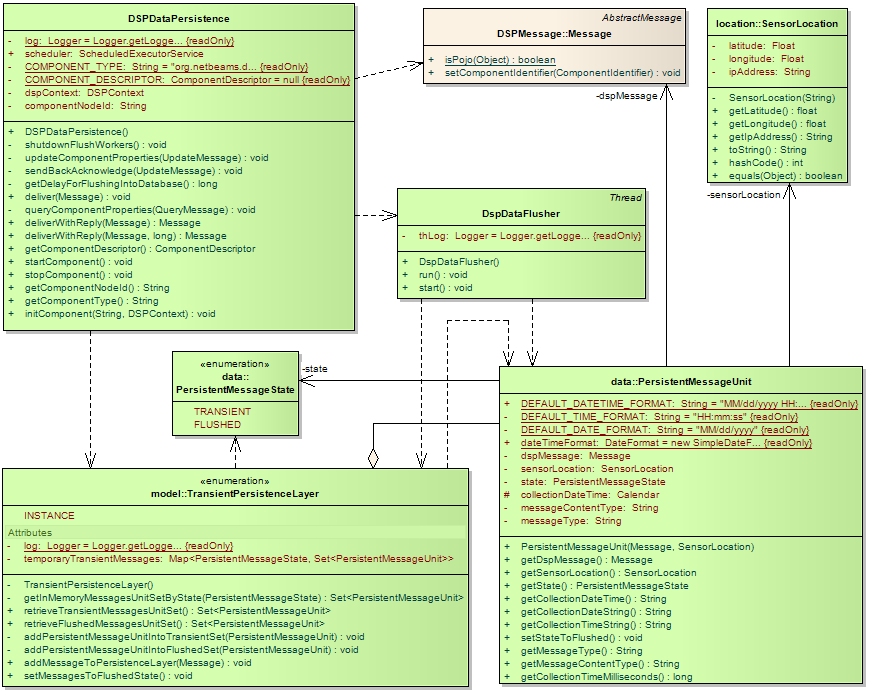
\includegraphics[scale=0.65]{../diagrams/DSP-DataPersistence-Flusher-Classes}
  \caption{UML Class diagram with DSP Data Persistence and Participating classes}
  \label{fig:DSP-DataPersistence-Flusher-Classes}
\end{figure}

Upon receiving a new DSP measurement message, the DSP Data Persistence
component keeps any received message in a temporary local cache, as described 
by the non-functional requirements. In this way, the DSP Data Persistence 
component maintains a dependency on the Singleton class TransientPersistenceLayer, 
responsible for encapsulating the DSP Message into an instance of the class 
PersistentMessageUnit, to be stored in the defined local cache.

According to the DSP Broker model described in \cite{netbeams-dsp-architecture}, 
the DSP Matcher needs to be updated with the addition of a matching rule that
filters a copy of any Measurement Message to the DSP Data Persistence component. 
As it is shown in Figure
\ref{fig:From-DSP-Broker-To-DSPDataPersistence-General-Sequence}, the worker
Thread DSP Data Flusher is the link between the Transient and Persistent
layers, as it depends on the references from the classes
TransientPersistenceLayer and the DSPMongoCRUDService.The class
DSPMongoCRUDService is responsible for extracting the collected data from the
body of the DSP Message and creating the keys designed to be persisted
in the mongoDB Database.

The DSP Broker retrieves the list of matching rules by contacting the Matcher.
As the DSP Platform has already loaded all the Matching rules, a copy of an
analyzed DSP Message is delivered to the DSP Data Persistence component specified
by a matcher rule. However, the UML Sequence Diagram depicted in Figure 
\ref{fig:From-DSP-Broker-To-DSPDataPersistence-General-Sequence} shows two 
different moments of message delivery:

\begin{figure}[!h]
  \centering
  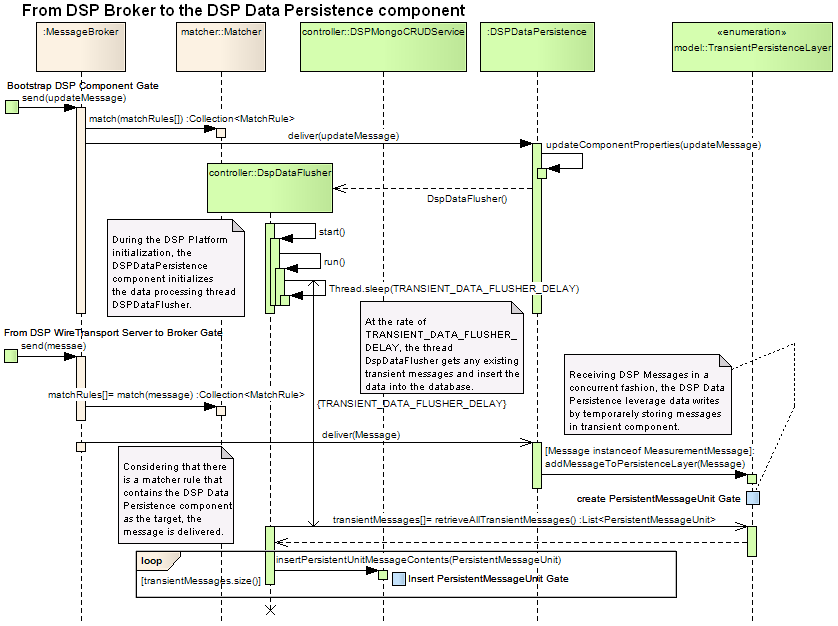
\includegraphics[scale=0.6]{../diagrams/From-DSP-Broker-To-DSPDataPersistence-General-Sequence} 
  \caption{UML Sequence Diagram - Flow 1: From the DSP Broker to the Data Persistence Component}
  \label{fig:From-DSP-Broker-To-DSPDataPersistence-General-Sequence}
\end{figure}

\begin{itemize}
  \item A bootstrap DSP Update Message is delivered to the DSP Data Persistence
  component when the DSP Platform is initializing the component. For example, the
  class DSPDataPersistence can initialize the class DspDataFlusher to
  flush temporary messages into the database at the rate of
  TRANSIENT\underline{ }DATA\underline{ }FLUSHER\underline{ }DELAY, defined in 
  seconds. 
  Listing \ref{file:dsp-data-persistence-bootstrap.xml}, on page
  \pageref{file:dsp-data-persistence-bootstrap.xml}, shows an implementation of
  a bootstrap message for the DSP Data Persistence;
  \item Any DSP Measure Message can be persisted by the DSP Data Persistence
  component. The component will add the message to a temporary memory location
  to decrease I/O on the database, when the DSP Broker delivers a DSP
  MeasureMessage to this component, as depicted by the UML Gate element
  \cite{uml-seq-gate} "create PersistentMessageUnit Gate". This last Gate
  describes the simple procedure to add the message into the transient
  persistent layer, as shown in Listing
  \ref{stream:dsp-message-serialized-ysi} on page
  \pageref{stream:dsp-message-serialized-ysi}.
\end{itemize}

The class PersistenceMessageUnit is the major transient persistence unit that
carries references regarding the originating DSP Message that was collected by
the DSP Data Persistence component. It is composed by an instance of the class 
SensorLocation and contains a reference to the PersistentMessageState
enumeration. The former identifies which sensor produced the collected data
from the DSP Message by the IP address, while the latter identifies whether
the PersistenceMessageUnit has been saved into the Database or not as depicted
by the UML State Diagram in Figure \ref{fig:PersistentMessageState-Diagram}. 
The class SensorLocation was developed as a to facilitate the identification of
sensor devices that are not capable of sampling their geographical location by
giving their references during the bootstrap process.

\begin{figure}[!h]
  \centering
  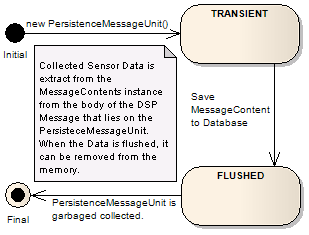
\includegraphics[scale=0.65]{../diagrams/PersistentMessageState-Diagram}
  \caption{UML State Diagram for the instance of the class
  PersistentMessageState}
  \label{fig:PersistentMessageState-Diagram}
\end{figure}

When a DSP Message is delivered to the DSP Data Persistence component, the
message is directly transferred to the Singleton class
TransientPersistenceLayer, as described before. As described in the UML
Sequence Diagram in Figure
\ref{fig:From-Create-PersistentMessageUnit-to-TransientPersistence-Layer-Sequence},
the first point of execution is the ``create PersistentMessageUnit Gate'',
where an instance of the SensorLocation is acquired for any DSP Message
received, in order to be added into the local cache. Before that occurs, the
PersistentMessageUnit is placed in the state ``TRANSIENT''.

\begin{figure}[!b]
  \centering
  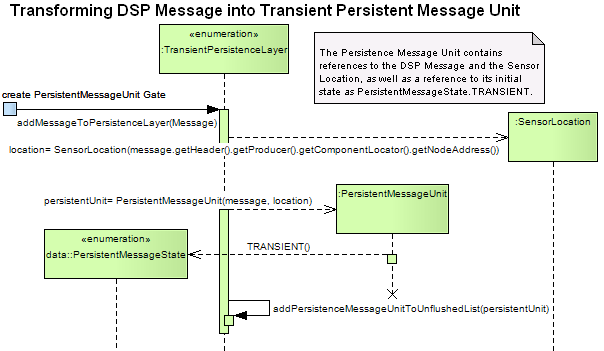
\includegraphics[scale=0.65]{../diagrams/From-Create-PersistentMessageUnit-to-TransientPersistence-Layer-Sequence}
  \caption{UML Sequence diagram - Adding a DSP Message into the Transient Persistence layer}
  \label{fig:From-Create-PersistentMessageUnit-to-TransientPersistence-Layer-Sequence}
\end{figure}

At this point, the DSP Data Persistence component maintains a set of DSP
Messages in a local cache during the specific ``flush rate'' specified in
the bootstrap message parameter. When the class DSPDataFlusher finds any number
of instances of PersistentMessageUnit in cache, it starts the process of
flushing them into the mongoDB database, described in the following section.

\subsection{Flushing data into the Database}

The class DSPDataFlusher is a thread designed to be in two different states, as
depicted in Figure \ref{fig:DSP-DataPersistence-Flusher-State-Diagram}:

\begin{figure}[!h]
  \centering
  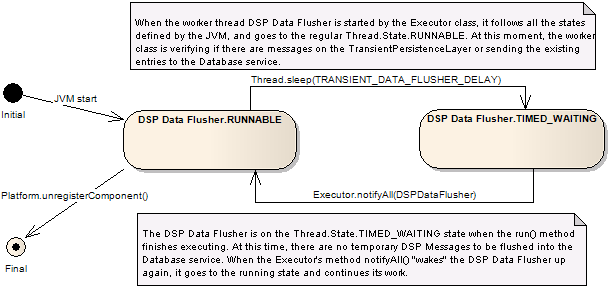
\includegraphics[scale=0.65]{../diagrams/DSP-DataPersistence-Flusher-State-Diagram}
  \caption{UML State diagram for the DSP Data Flusher Worker Thread}
  \label{fig:DSP-DataPersistence-Flusher-State-Diagram}
\end{figure}

\begin{itemize}
  \item \textbf{Waiting}: the initial state of a Java thread
  after its initialization, waiting to be on the ``runnable'' state. This
  period of time is defined by the ``flush rate''  specified in the bootstrap
  message of the DSP Data Persistence component;
  \item \textbf{Running}: the class DSPDataFlusher contacts the class
  TransientPersistenceLayer, in order to verify if there are any instance of
  the class PersistentMessageUnit waiting to be transmitted from the temporary
  cache to the Database service. If the cache is not empty, the DSPDataFlusher 
  acquires the lock over the TransientPersistenceLayer and retrieves the
  existing set of PersistentMessageUnit to be sent to mongoDB. Then, it sends
  all of the PersistentMessageUnit classes to the Singleton Service class 
  DSPMongoCRUDService, which is responsible to extract the collected data from
  the DSP Message's Body and convert it to the Key-Value model specified in
  Section \ref{sec:dsp-persistence-data-model}.
\end{itemize}

The main participating classes from the DSPMongoCRUDService are shown in the
UML Class Diagram \ref{fig:DSP-Data-Persistence-Mongo-Classes}. It keeps references
to all types of sensor devices. Furthermore, it is responsible to implement the
CRUD methods to modify the mongoDB database state. The class Mongo is used to acquire
an instance of the connection with mongoDB server and provide Factory Methods 
\cite{gof} to create instances of the classes DB, DBCollection and
BasicDBObject. The class DB is used as a reference to a database namespace, 
such as ``netbeams'', the one suggested and implemented by this work. Similarly,
class DBCollection offers an API to manipulate similar documents via the
abstraction of a collection of items. Finally, the class BasicDBObject is used
to represent the keys and values to be persisted in the database.

\begin{figure}[!h]
  \centering
  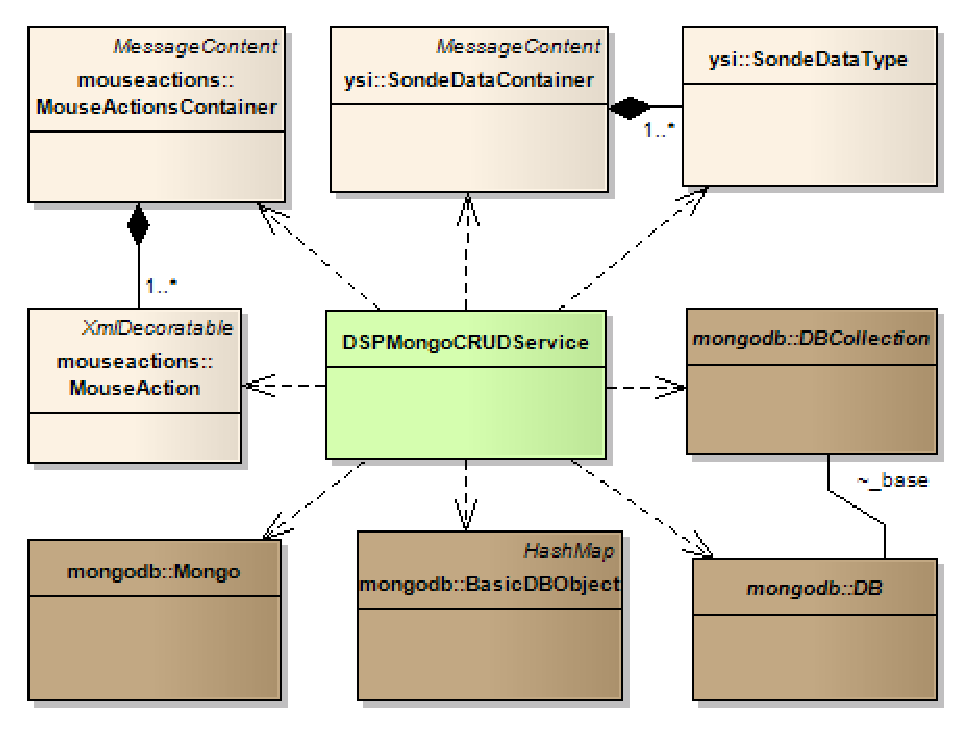
\includegraphics[scale=0.65]{../diagrams/DSP-Data-Persistence-Mongo-Classes}
  \caption{UML Class diagram with Persistence Service for MongoDB}
  \label{fig:DSP-Data-Persistence-Mongo-Classes}
\end{figure}

The last method call of the UML Sequence Diagram, depicted in Figure
\ref{fig:From-DSP-Broker-To-DSPDataPersistence-General-Sequence}, shows the
method call to the DSPMongoCRUDService method call to persist each of the
PersistentMessageUnit (see execution point ``addPersistentMessageUnit Gate'').
In short, the class DspDataFlusher continuously wakes up at the rate of
``TRANSIENT\underline{ }DATA\underline{ }FLUSHER\underline{ }DELAY''. Its
purpose is as simple as to iterate over the list of PersitenceMessageUnit on
the state of TRANSIENT, and send each of them to be saved on the persistence
storage. 

Finally, this sequence of events is continued by "inserting''
``PersistenceMessageUnit Gate", which triggers the persistence service from the
chosen database system as shown in Figure
\ref{fig:From-Insert-PersistentMessageUnit-to-mongoDB}.

\begin{figure}[!h]
  \centering
  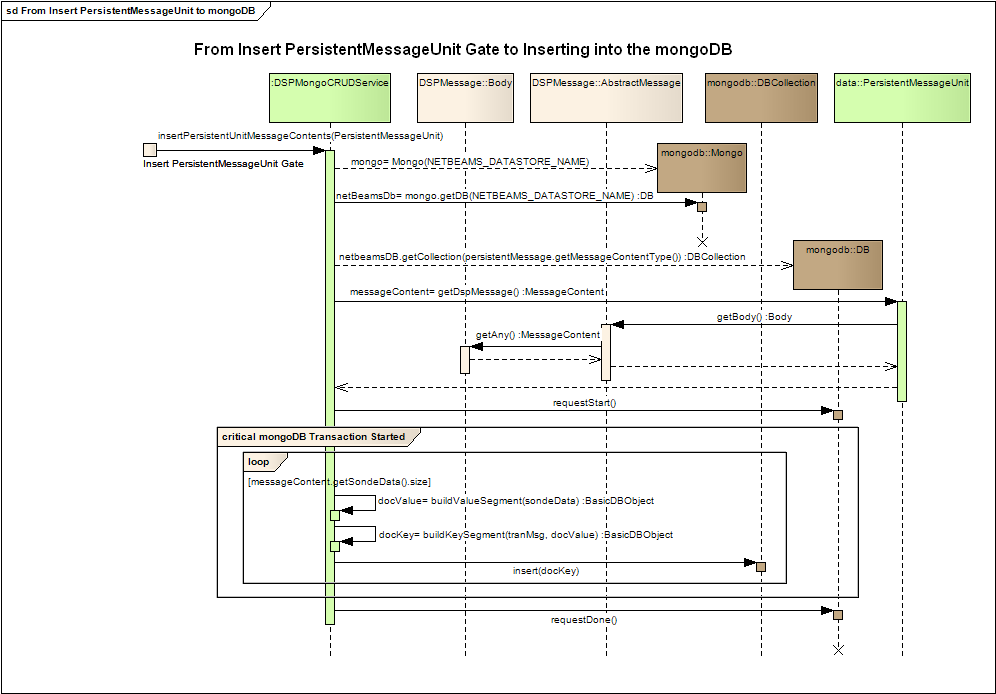
\includegraphics[scale=0.6]{../diagrams/From-Insert-PersistentMessageUnit-to-mongoDB} 
  \caption{UML Sequence Diagram - MessageContent instance saved by the class
  mongoDB service}
  \label{fig:From-Insert-PersistentMessageUnit-to-mongoDB}
\end{figure}

\subsubsection{Creating mongoDB Document instance of Key-Values}

In order to build the mongoDB document described in section
\ref{sec:dsp-persistence-data-model}, the reference to the DSP Message is
used to extracted the metadata, while the reference to the DSP Message Content 
from the body of the DSP Message is used to extract the collected data from
sensors.

\begin{figure}[!h]
  \centering
  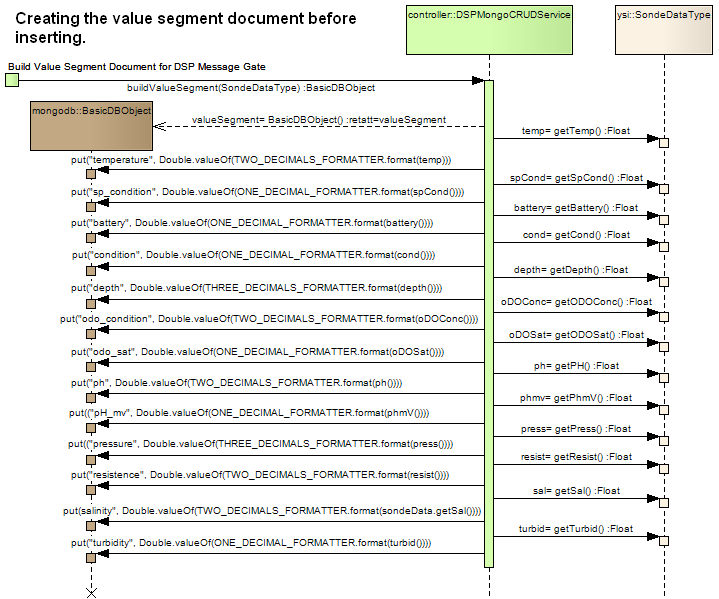
\includegraphics[scale=0.6]{../diagrams/From-Creating-Value-Segment-Sequence}
  \caption{UML Sequence diagram showing the creation of the keys for the
  collected data}
  \label{fig:From-Creating-Value-Segment-Sequence}
\end{figure}

\newpage

After the keys for the collected data are created, the keys for the metadata
are captured as shown in the UML Sequence Diagram in Figure
\ref{fig:From-Creating-Key-Segment-Sequence}.

\begin{figure}[!h]
  \centering
  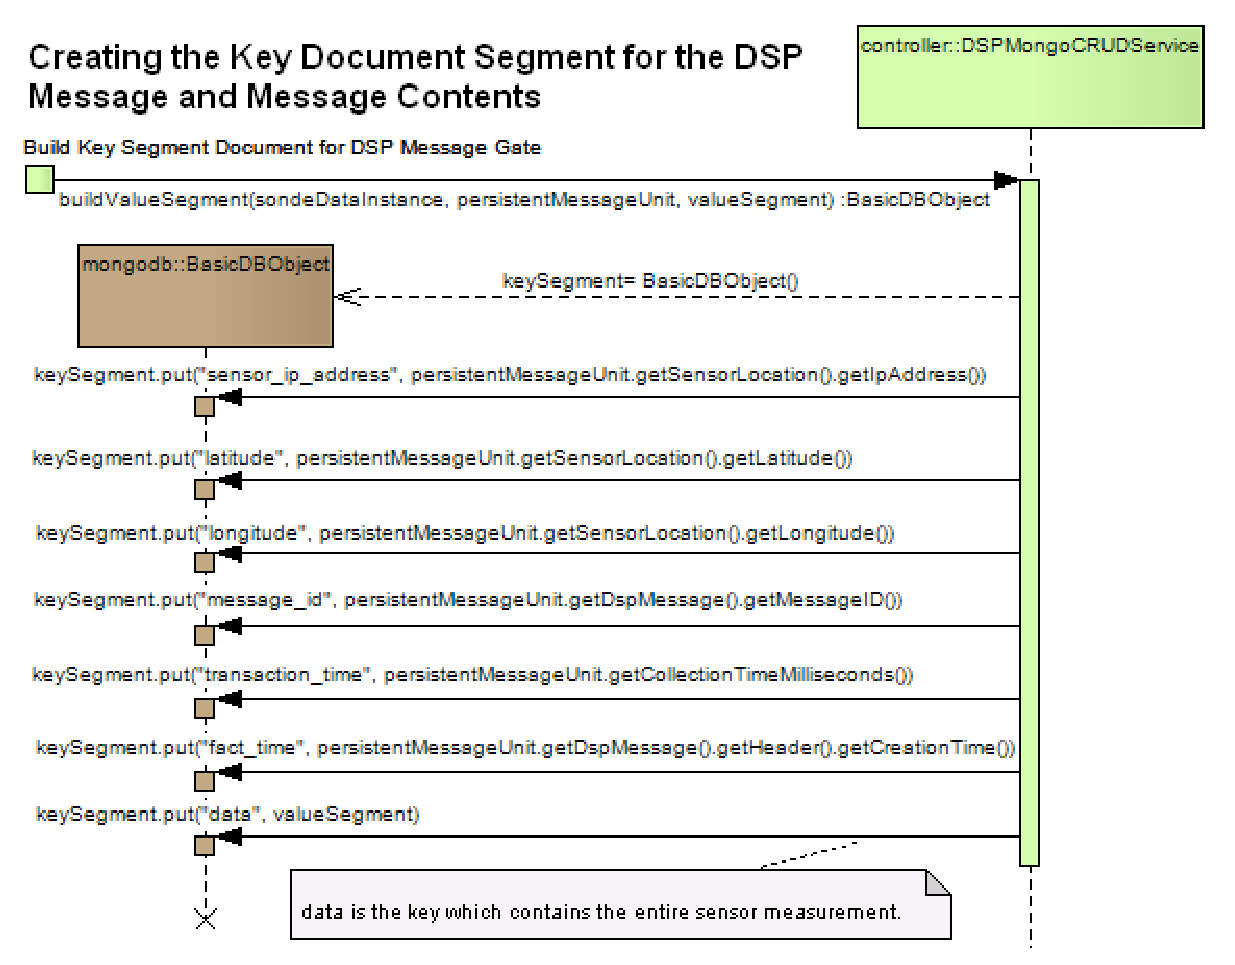
\includegraphics[scale=0.65]{../diagrams/From-Creating-Key-Segment-Sequence}
  \caption{UML Sequence diagram showing the creation of the keys for the
  metadata}
  \label{fig:From-Creating-Key-Segment-Sequence}
\end{figure}

To summarize, the DSP Data Persistence Component is added into the DSP Platform
by introducing a new component that provides service to the transfer any
collected data from sensor devices to mongoDB, the Key-Value Pair database
technology. The general dependencies of the system can be seen in UML
Class Diagram depicted by Figure \ref{fig:DSP-Data-Persistence-Classes}, that
expands the UML Package Dependency Diagram shown in Figure
\ref{fig:DSP-Data-Persistence-Packages-Dependency}.

\begin{figure}[!t]
  \centering
  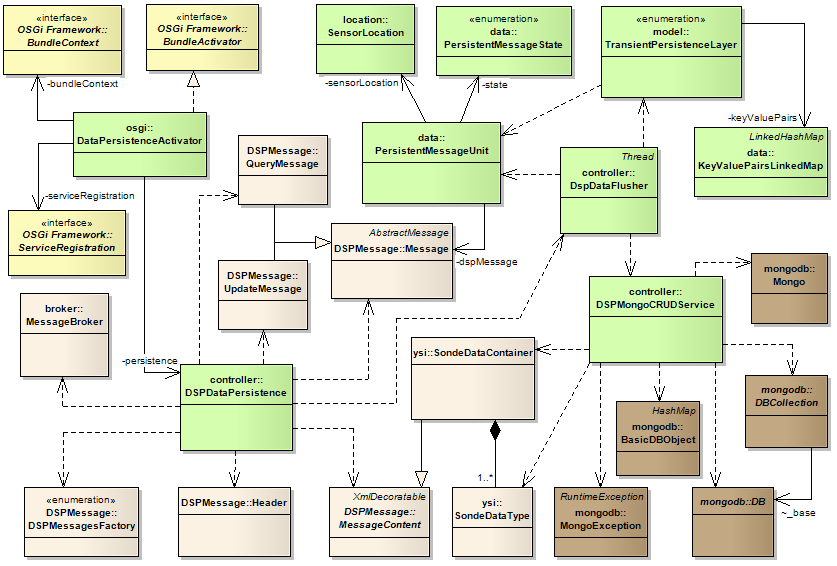
\includegraphics[scale=0.65]{../diagrams/DSP-Data-Persistence-Classes}
  \caption{UML Class diagram for the DSP Data Persistence component.}
  \label{fig:DSP-Data-Persistence-Classes}
\end{figure}

Next section analyzes the deployment details for the DSP Platform and the
mongoDB integration.

\subsection{DSP Data Persistence Deployment}

The deployment of the persistence layer is accomplished by the addition of two
new components to the DSP Platform: the DSP Data Persistence component and MongoDB
Database Server. The DSP Data Persistence component is responsible for capturing 
any data produced by sensors in the data sink, while mongoDB is where the data is 
going to be stored, as a result of the technology selection on the previous chapter. 

The deployment of the DSP Data Persistence follows the deployment specifications
of a DSP Component over an OSGi Framework. For the development of this work,
the Knopflerfish OSGi Container \cite{knopflerfish} was used. The details of the
implementation are described in Section
\ref{sec:dsp-data-persistence-implementation}. The deployment of the mongoDB
can be accomplished in different approaches, summarized as follows:

\begin{itemize}
  \item \textbf{Single Server}: a regular deployment of a database system as it
  is done in general applications, where data is managed by one single process;
  \item \textbf{Sharded Server}: a deployment approach where data is sharded
  into different servers.
\end{itemize} 

The single server approach maintains all data located in a simple space.
Distributed Systems applications such as Master-Slave, Data Replication, etc
can be used in this approach for scalability
\ref{fig:DSP-Data-Persistence-Deployment-Single}. 

\begin{figure}[!h]
  \centering
  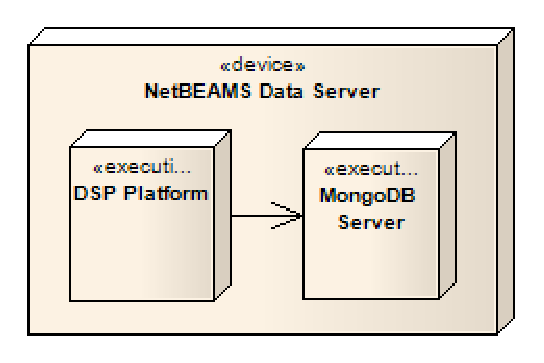
\includegraphics[scale=0.7]{../diagrams/DSP-Data-Persistence-Deployment-Single}
  \caption{UML Deployment diagram with a single server}
  \label{fig:DSP-Data-Persistence-Deployment-Single}
\end{figure}

Given that mongoDB provides support for Database Partitioning by using
the concept of Shards, the implementation of a Data-Centric approach can be done
by deploying different mongoDB instances in a distributed cluster, where each
node can hold different collections of data. mongoDB provides Horizontal
Partition with automatic distribution based on the ranges of a given key of
the document. For NetBEAMS collected data, a good candidate for partitioning is
the time when the data was created, and separate each shard in groups of months
of the year.

\begin{figure}[!h]
  \centering
  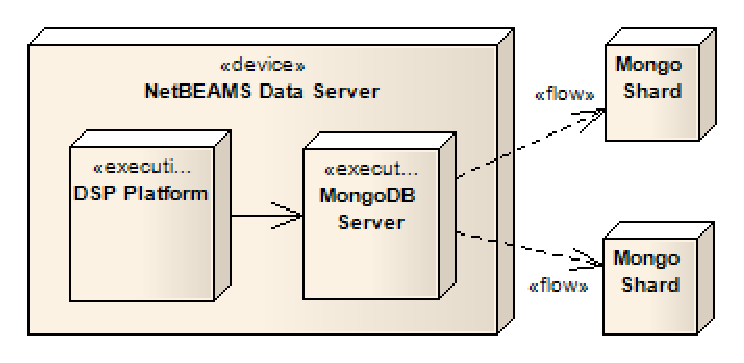
\includegraphics[scale=0.7]{../diagrams/DSP-Data-Persistence-Deployment-Sharded}
  \caption{UML Deployment Diagram for a sharded server}
  \label{fig:DSP-Data-Persistence-Deployment-Sharded}
\end{figure}

The design of the DSP Data Persistence uses the DSP Component specification
defined by the DSP Platform. First, the analysis of the business process
helped to understand the requirements of the system. The data model design
followed the specifications defined in Chapter 5. Each of the layers of the
system was described using UML Diagrams, having partial details regarding the
OSGi implementation. The next chapter entails the experiments conducted to
evaluate the designs discussed in this chapter, and walks through the
experiments conducted to verify the implementation of using mongoDB.
